\documentclass[a4paper]{article}
\usepackage[utf8]{inputenc}
\usepackage{indentfirst}
\usepackage{float}
\usepackage{geometry}
\usepackage{polski}
\usepackage{mathtools}
\usepackage{tcolorbox}
\usepackage{listings}
\usepackage{amssymb}
\usepackage[none]{hyphenat}
\usepackage{tabularx}
\usepackage{tikz}
\usepackage{array}
\usepackage{booktabs,adjustbox}

\renewcommand{\familydefault}{\sfdefault}
\newcommand\tab[1][1cm]{\hspace*{#1}}
\lstset{frame=tb,
  language=Java,
  aboveskip=3mm,
  belowskip=3mm,
  showstringspaces=false,
  columns=flexible,
  basicstyle={\small\ttfamily},
  numbers=none,
  numberstyle=\tiny\color{rgb}{0.5,0.5,0.5},
  keywordstyle=\color{rgb}{0.58,0,0.82}
  commentstyle=\color{rgb}{0,0.6,0},
  stringstyle=\color{mauve},
  breaklines=true,
  breakatwhitespace=true,
  tabsize=3
}

\title{\textbf{VaccDistributor}}
\author{Kamil Sztandur}
\date{14/11/2020}
\begin{document}
\begin{tcolorbox}
\maketitle
\end{tcolorbox}
\centerline{\textbf{SPECYFIKACJA IMPLEMENTACYJNA}}
\newpage

\section*{\underline{Rozdział 1:  INFORMACJE OGÓLNE.}}
\subsection*{Podrozdział 1.1: Nazwa programu.}
\tab Program nazywa się \textbf{VaccDistributor}.

\subsection*{Podrozdział 1.2: Poruszany problem.}
\tab Problemem rozwiązywanym przez ten program jest zagadnienie jak najbardziej optymalnego pod kątem ekonomicznym rozdysponowania szczepionek pomiędzy poszczególnymi dostawcami, a aptekami, na podstawie podanych przez użytkownika połączeń. Program skupia się na tym, aby koszt dystrybucji szczepionek był jak najmniejszy. Nie gwarantuje, że zapotrzebowanie każdej apteki zostanie zaspokojone. Także jest to wariant egoistyczny.

\subsection*{Podrozdział 1.3: Uruchomienie programu.}
\tab Uruchomienie programu ze względu na brak oprawy graficznej może sprawiać trudności mniej wtajemniczonym w komputery użytkownikom. Program uruchamia się z poziomu terminalu systemu operacyjnego, na którym jest zainstalowana najnowsza wersja oprogramowania Java. Aby uruchomić program wystarczy wpisać komendę w terminalu systemu operacyjnego spełniającego opisane wymagania:
\begin{lstlisting}
	java -jar vaccDistributor.jar input.txt
\end{lstlisting}
znajdując się w katalogu, w którym umieszczone zostały równocześnie plik programu \textbf{vaccDistributor.jar} oraz tekstowy plik wejściowy z danymi (tutaj \textbf{input.txt}). Należy pamiętać o dopisaniu rozszerzenia pliku. Sama nazwa (tutaj \textbf{input}) nie pozwoliłaby na odnalezienie wskazanego pliku. \newline \newline
\tab Należy dokładnie przestudiować strukturę pliku wejściowego na podstawie poniższego przykładu, ponieważ wszelkie odstępstwa od ogólnoprzyjętego szablonu mogą spowodować nieprawidłową pracę, a nawet zatrzymanie pracy programu. Tekstowy plik wejściowy powinien zawierać trzy nagłówki, oznaczające kolejno listy producentów, aptek i dostępnych połączeń. Kolejne parametry w linijce powinny być oddzielna ciągiem znaków " $|$ ". Nie należy powielać nagłówków ani umieszczać ich w innej kolejności.
\newline
\newline \textbf{Przykładowy plik wejściowy:}
\begin{tcolorbox}
\# Producenci szczepionek (id | nazwa | dzienna produkcja)
\newline 0 $|$ BioTech 2.0 $|$ 900
\newline 1 $|$ EkoPolska 2020 $|$ 1300
\newline \# Apteki (id $|$ nazwa $|$ dzienne zapotrzebowanie)
\newline 0 $|$ CentMedEko Centrala $|$ 450 
\newline 1 $|$ CentMedEko 24h $|$ 690 
\newline \# Połączenia producentów i aptek (id producenta $|$ id apteki $|$ dzienna maksymalna liczba dostarczanych szczepionek $|$ koszt szczepionki [zł] )
\newline 0 $|$ 0 $|$ 800 $|$ 70.5 
\newline 0 $|$ 1 $|$ 600 $|$ 70 
\newline 1 $|$ 0 $|$ 900 $|$ 100 
\newline 1 $|$ 1 $|$ 600 $|$ 80
\end{tcolorbox}
\newpage

\section*{\underline{Rozdział 2: OPIS MODUŁÓW I PAKIETÓW.}}
\begin{figure}[H]
    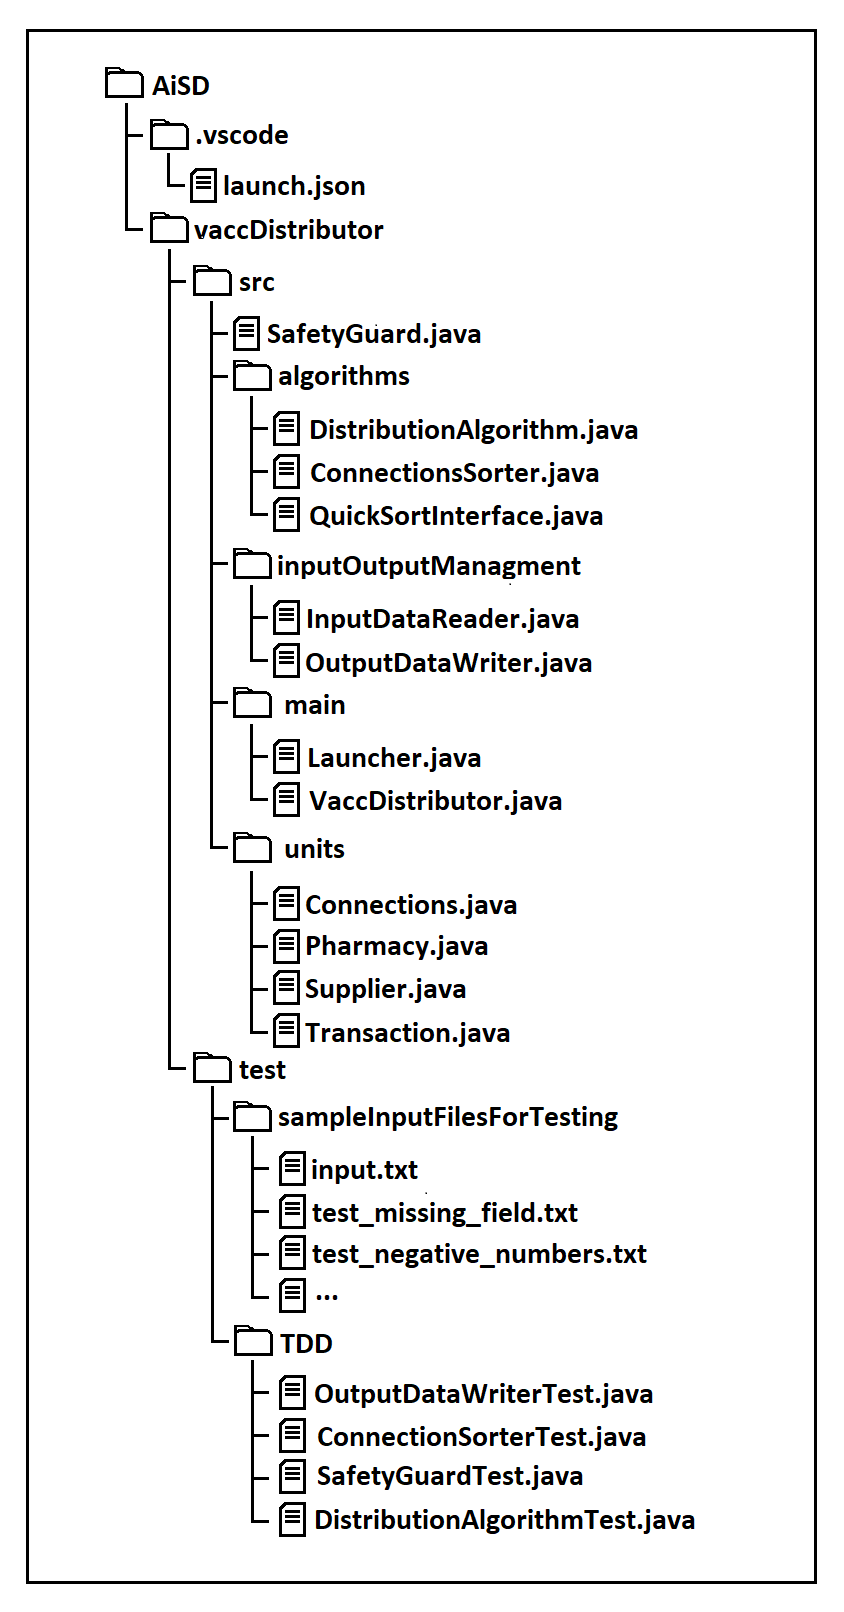
\includegraphics[width=10cm]{Katalogi.png}
    \centering
\end{figure}
\newpage

\subsection*{Podrozdział 2.1: PAKIET 'vaccDistributor'}
Ten pakiet jest głównym pakietem programu. Zawiera jedynie dwa podpakiety odpowiadające za logikę oraz testowanie programu:
\begin{itemize}
\item \textbf{src -} pakiet stanowiący całą logikę programu. 
\item \textbf{test -} pakiet odpowiedzialny za testowanie programu.
\end{itemize}

\subsection*{Podrozdział 2.1.1: PAKIET 'vaccDistributor.src'}
Ten pakiet zawiera całą logikę programu, czyli podpakiety odpowiadające za pewne segmenty programu oraz klasę ds. bezpieczeństwa pracy programu:
\begin{itemize}
\item \textbf{SafetyGuard.java -} klasa stanowiąca zbiór metod pozwalających kontrolować bezpieczeństwo przebiegu programu, wykorzystywana we wszystkich podpakietach pakietu src.
\item \textbf{algorithms -} podpakiet zawierający algorytmy zastosowane w programie.
\item \textbf{inputOutputManagment -} podpakiet zawierający zbiór obiektów zajmujących się wyjściem/wejściem w programie.
\item \textbf{main -} podpakiet zawierający główne ciało programu, zarządzające i korzystające z pozostałych pakietów i obiektów programu.
\item \textbf{units -} podpakiet zawierający obiekty jednostek używanych w programie przedstawiających interesujące nas realne obiekty.
\end{itemize}

\subsection*{Podrozdział 2.1.1.1: PAKIET 'vaccDistributor.src.algorithms'}
Podpakiet zawierający algorytmy zastosowane w programie.
\begin{itemize}
\item \textbf{DistributionAlgorithm.java -} klasa zawierająca algorytm tworzący najbardziej ekonomiczne (tanie) połączenia pomiędzy producentami szczepionek, a aptekami.
\item \textbf{ConnectionsSorter.java -} klasa zawierająca algorytm sortowania połączeń (używany przez główny algorytm programu) bazujący na sortowaniu szybkim QuickSort.
\item \textbf{QuickSortInterface.java -} interfejs pomocniczy i pilnujący bezpieczeństwa właściwego formatu sortowania szybkiego w algorytmie sortowania połączeń.
\end{itemize}

\subsection*{Podrozdział 2.1.1.2: PAKIET 'vaccDistributor.src.inputOutputManagment'}
Podpakiet zawierający klasy zajmujące się wejściem i wyjściem w programie.
\begin{itemize}
\item \textbf{InputDataReader.java -} klasa odpowiedzialna za czytanie danych podanych przez użytkownika i utworzenie z nich możliwych do pobrania z tej klasy 'kontenerów' z przeczytanymi danymi.
\item \textbf{OutputDataWriter.java -} klasa odpowiedzialna za utworzenie katalogu z danymi wyjściowymi oraz wypisywanie danych wyjściowych (najbardziej optymalnych połączeń z aptekami) do pliku tekstowego w utworzonym katalogu.
\end{itemize}

\subsection*{Podrozdział 2.1.1.3: PAKIET 'vaccDistributor.src.main'}
Podpakiet zawierający główne ciało programu. Korzysta ono z pozostałych obiektów i pakietów dostępnych w ramach pakietu \textbf{src}.
\begin{itemize}
\item \textbf{Launcher.java -} klasa zawierająca główną metodę \textbf{main}, która odpowiada tylko za uruchomienie programu.
\item \textbf{VaccDistributor.java -} klasa zawierające główne ciało programu, realizujące krok po kroku wszystkie wymagania biznesowe programu.
\end{itemize}

\subsection*{Podrozdział 2.1.1.4: PAKIET 'vaccDistributor.src.units'}
Podpakiet zawierający obiekty jednostek używanych w programie przedstawiających interesujące nas realne obiekty takie jak apteki czy producentów. To na nich pracuje algorytm ustalający dystrybucję szczepionek.
\begin{itemize}
\item \textbf{Supplier.java -} klasa stanowiąca reprezentację producenta szczepionek (in. dostawcy) w programie.
\item \textbf{Pharmacy.java -} klasa stanowiąca reprezentację placówkę apteki w programie.
\item \textbf{Connection.java -} klasa stanowiąca reprezentację połączenia producent - apteka w programie.
\item \textbf{Transaction.java -} klasa stanowiąca reprezentację optymalnego połączenia ustalonego przez algorytm, która jest de facto umową na dostarczenie pewnej ilości szczepionek za pewną cenę danym połączeniem, bazującym na istniejącej klasie \textbf{Connection}.
\end{itemize}

\subsection*{Podrozdział 2.1.2: PAKIET 'vaccDistributor.test'}
Pakiet zawierający pakiet i katalog z przykładowymi danymi wejściowymi. Pozwala na testowanie manualne i automatyczne programu.
\begin{itemize}
\item \textbf{sampleInputFilesForTesting -} nie jest to pakiet, lecz katalog zawierający zestaw przykładowych danych wejściowych w tym poprawnych i błędnych.
\item \textbf{TDD -} pakiet zawierający zestaw klas oferujących zbiór testów jednostkowych, testujących metody i klasy oferowane przez pakiet \textbf{src}.
\end{itemize}

\subsection*{Podrozdział 2.1.2.1: PAKIET 'vaccDistributor.test.TDD'}
Pakiet zawierający zestaw klas oferujących zbiór testów jednostkowych, testujących metody i klasy oferowane przez pakiet \textbf{src}.
\begin{itemize}
\item \textbf{OutputDataWriter.java -} klasa testująca oferująca szereg metod sprawdzających poprawność działania klasy OutputDataWriter z pakietu \textbf{vaccDistributor.src.inputOutputManagment}.
\item \textbf{ConnectionsSorterTest.java -} klasa testująca oferująca szereg metod sprawdzających poprawność działania algorytmu QuickSort z klasy ConnectionsSorter z pakietu\newline \textbf{vaccDistributor.src.inputOutputManagment}.
\item \textbf{SafetyGuardTest.java -} klasa testująca oferująca szereg metod sprawdzających skuteczność klasy ds. bezpieczeństwa pracy programu SafetyGuard z pakietu \textbf{vaccDistributor.src}.
\item \textbf{DistributionAlgorithmTest.java -} klasa testująca oferująca szereg metod sprawdzających poprawność działania algorytmu rozdysponowującego szczepionki i ustalającego jak najbardziej ekonomicznie optymalne połączenia aptek z producentami, czyli klasy DistributionAlgorithm z pakietu \textbf{vaccDistributor.src.algorithms}.
\end{itemize}

\section*{\underline{Rozdział 3: OPIS KLAS.}}
\subsection*{Podrozdział 3.1: KLASA 'SafetyGuard'}
\begin{flushleft}
Klasa stanowiąca zbiór metod pozwalających kontrolować bezpieczeństwo przebiegu programu, wykorzystywana we wszystkich podpakietach pakietu \textbf{src}. Nie potrzebuje konstruktora. Zawiera jedynie statyczne metody.
\end{flushleft} 

\centerline{
\begin{tabular}{| p{3.5cm} | p{5cm} | p{4cm} | m{2cm} |} 
\toprule
\multicolumn{1}{l}{\textbf{NAZWA METODY}} & 
\multicolumn{1}{l}{\textbf{OPIS METODY}} & 
\multicolumn{1}{l}{\textbf{PARAMETRY METODY}} & 
\multicolumn{1}{r}{\textbf{\parbox[t]{2cm}{ZWRACANA WARTOŚĆ}}} \\ 
\midrule
\hline
\parbox[t]{3cm}{areConnectionsEfficient\\EnoughForThisPharmacy} & 
\parbox[t]{5cm}{Metoda sprawdzająca, czy połączenia do danej apteki są z góry skazane na niemożność ich zaopatrzenia} & 
\parbox[t]{4cm}{Pharmacy$:$pharmacy,\\ ArrayList$<$Connection$>$:\\connections} &
\parbox[t]{2cm}{boolean} \\ \hline

\parbox[t]{3cm}{checkIfSupplierData\\LineCorrect} & 
\parbox[t]{5cm}{Metoda sprawdzająca, czy wyczytany w pliku wiersz z danymi producenta jest poprawny. Rzuca wyjątek IAEx, jeżeli nie.} & 
\parbox[t]{4cm}{String$[]$:dataLine,\\ int:lineNumber} &
\parbox[t]{2cm}{void} \\ \hline

\parbox[t]{3cm}{checkIfPharmacyData\\LineCorrect} & 
\parbox[t]{5cm}{Metoda sprawdzająca, czy wyczytany w pliku wiersz z danymi apteki jest poprawny. Rzuca wyjątek IAEx, jeżeli nie.} & 
\parbox[t]{4cm}{String$[]$:dataLine,\\ int:lineNumber} &
\parbox[t]{2cm}{void} \\ \hline

\parbox[t]{3cm}{checkIfConnectionData\\LineCorrect} & 
\parbox[t]{5cm}{Metoda sprawdzająca, czy wyczytany w pliku wiersz z danymi połączenia jest poprawny. Rzuca wyjątek IAEx, jeżeli nie.} & 
\parbox[t]{4cm}{String$[]$:dataLine,\\ int:lineNumber} &
\parbox[t]{2cm}{void} \\ \hline

\parbox[t]{3cm}{isThisPharmacy\\Duplicated} & 
\parbox[t]{5cm}{Metoda sprawdzająca, czy podana apteka jest duplikatem jakiejś już wczytanej.} & 
\parbox[t]{4cm}{Pharmacy : newPharmacy,\\ HashMap$<$Integer, Pharmacy$>$ : pharmacies} &
\parbox[t]{2cm}{boolean} \\ \hline

\parbox[t]{3cm}{isThisSupplier\\Duplicated} & 
\parbox[t]{5cm}{Metoda sprawdzająca, czy podany producent jest duplikatem jakiegoś już wczytanego.} & 
\parbox[t]{4cm}{Supplier : newSupplier,\\ HashMap$<$Integer, Supplier$>$ : suppliers} &
\parbox[t]{2cm}{boolean} \\ \hline

\parbox[t]{3cm}{isThisConnection\\Duplicated} & 
\parbox[t]{5cm}{Metoda sprawdzająca, czy podane połączenie jest duplikatem jakiegoś już wczytanego.} & 
\parbox[t]{4cm}{Connection: newConnection,\\ ArrayList$<$Connection$>$: connections} &
\parbox[t]{2cm}{boolean} \\ \hline

\parbox[t]{3cm}{isThisTransaction\\Duplicated} & 
\parbox[t]{5cm}{Metoda sprawdzająca, czy podana transakcja jest duplikatem jakiejś już ustalonej przez algorytm} & 
\parbox[t]{4cm}{Transaction: newTransaction,\\ ArrayList$<$Transaction$>$: transactions} &
\parbox[t]{2cm}{boolean} \\ \hline

\parbox[t]{3cm}{isThisConnection\\PharmacyRegistered} & 
\parbox[t]{5cm}{Metoda sprawdzająca, czy apteka do której prowadzi podane połączenie istnieje na liście wczytanych aptek.} & 
\parbox[t]{4cm}{Connection: connection,\\HashMap$<$Integer, Pharmacy$>$: pharmacies} &
\parbox[t]{2cm}{boolean} \\ \hline

\parbox[t]{3cm}{isThisConnection\\SupplierRegistered} & 
\parbox[t]{5cm}{Metoda sprawdzająca, czy producent od którego prowadzi podane połączenie istnieje na liście wczytanych producentów.} & 
\parbox[t]{4cm}{Connection: connection,\\HashMap$<$Integer, Supplier$>$: suppliers} &
\parbox[t]{2cm}{boolean} \\ \hline
\end{tabular}
}
\newpage

\subsection*{Podrozdział 3.2: KLASA 'InputDataReader'}
\begin{flushleft}
Klasa odpowiedzialna za czytanie danych podanych przez użytkownika i utworzenie z nich możliwych do pobrania z tej klasy 'kontenerów' z przeczytanymi danymi. Konstruktor przyjmuje zmienną typu String z nazwą pliku wejściowego.
\end{flushleft} 
\textbf{ATRYBUTY:}
\begin{itemize}
\item \textbf{private String inputFilename -} zmienna przechowująca nazwę pliku wejściowego z danymi podanego przez użytkownika.
\item \textbf{private HashMap<Integer, Supplier> suppliers -} kontener przechowujący wczytanych producentów z pliku wejściowego.
\item \textbf{private HashMap<Integer, Pharmacy> pharmacies -} kontener przechowujący wczytane apteki z pliku wejściowego.
\item \textbf{private ArrayList<Connection> connections -} kontener przechowujący wczytane połączenia z pliku wejściowego.
\item \textbf{private boolean suppliersListHasBeenRead -} flaga określająca, czy pole z listą producentów zostało przeczytane. Służy do wykrywania zduplikowanych pól w pliku.
\item \textbf{private boolean pharmaciesListHasBeenRead -} flaga określająca, czy pole z listą aptek zostało przeczytane. Służy do wykrywania zduplikowanych pól w pliku.
\item \textbf{private boolean connectionsListHasBeenRead -} flaga określająca, czy pole z listą połączeń zostało przeczytane. Służy do wykrywania zduplikowanych pól w pliku.
\end{itemize}

\centerline{
\begin{tabular}{| p{3.5cm} | p{5cm} | p{1cm} | m{5cm} |} 
\toprule
\multicolumn{1}{l}{\textbf{NAZWA METODY}} & 
\multicolumn{1}{l}{\textbf{OPIS METODY}} & 
\multicolumn{1}{l}{\textbf{PARAMETRY METODY}} & 
\multicolumn{1}{r}{\textbf{\parbox[t]{2cm}{ZWRACANA WARTOŚĆ}}} \\ 
\midrule
\hline
\parbox[t]{3cm}{read} & 
\parbox[t]{5cm}{Metoda czytająca plik, którego nazwę podano w konstruktorze. Wczytuje do odpowiednich kontenerów wyczytane dane z pliku. Rzuca wyjątek w przypadku błędu.} & 
\parbox[t]{1cm}{void} &
\parbox[t]{5cm}{void} \\ \hline

\parbox[t]{3cm}{getSuppliers} & 
\parbox[t]{5cm}{Metoda zwracająca HashMapę z wyczytanymi producentami.} & 
\parbox[t]{1cm}{void} &
\parbox[t]{5cm}{HashMap$<$Integer, Supplier$>$} \\ \hline

\parbox[t]{3cm}{getPharmacies} & 
\parbox[t]{5cm}{Metoda zwracająca HashMapę z wyczytanymi aptekami.} & 
\parbox[t]{1cm}{void} &
\parbox[t]{5cm}{HashMap$<$Integer, Pharmacy$>$} \\ \hline

\parbox[t]{3cm}{getConnections} & 
\parbox[t]{5cm}{Metoda zwracająca ArrayListę z wyczytanymi połączeniami.} & 
\parbox[t]{1cm}{void} &
\parbox[t]{5cm}{ArrayList$<$Connection$>$} \\ \hline

\parbox[t]{3cm}{readRecordFor} & 
\parbox[t]{5cm}{Metoda prywatna używana przez read() czytająca bieżącą linijkę i zapisującą uzyskaną daną do odpowiedniego kontenera na podstawie parametru nowReading.} & 
\parbox[t]{1cm}{String:nowReading,\\ String:line, int:lineNumber} &
\parbox[t]{5cm}{void} \\ \hline

\parbox[t]{3cm}{getInputFile} & 
\parbox[t]{5cm}{Metoda prywatna używana przez read() zwracająca wskaźnik do pliku z danymi wejściowymi lub rzucająca wyjątek, jeżeli plik nie istnieje.} & 
\parbox[t]{1cm}{void} &
\parbox[t]{5cm}{File} \\ \hline
\end{tabular}
}
\newpage

\subsection*{Podrozdział 3.3: KLASA 'OutputDataWriter'}
\begin{flushleft}
Klasa odpowiedzialna za utworzenie katalogu z danymi wyjściowymi oraz wypisywanie danych wyjściowych (najbardziej optymalnych połączeń z aptekami) do pliku tekstowego w utworzonym katalogu. W konstruktorze przyjmuje nazwę, którą ma przyjąć plik z danymi wyjściowymi.
\end{flushleft} 
\textbf{ATRYBUTY:}
\begin{itemize}
\item \textbf{private String directoryName -} zmienna przechowująca nazwę katalogu z danymi wyjściowymi.
\item \textbf{private String filename -} zmienna przechowująca nazwę pliku tekstowego z danymi wyjściowymi.
\end{itemize}

\centerline{
\begin{tabular}{| p{3.5cm} | p{5cm} | p{3cm} | m{2cm} |} 
\toprule
\multicolumn{1}{l}{\textbf{NAZWA METODY}} & 
\multicolumn{1}{l}{\textbf{OPIS METODY}} & 
\multicolumn{1}{l}{\textbf{PARAMETRY METODY}} & 
\multicolumn{1}{r}{\textbf{\parbox[t]{2cm}{ZWRACANA WARTOŚĆ}}} \\ 
\midrule
\hline
\parbox[t]{3cm}{createOutputDir} & 
\parbox[t]{5cm}{Metoda tworząca katolog z rozwiązaniem. Rzuca wyjątek IOEx w przypadku problemu.} & 
\parbox[t]{3cm}{void} &
\parbox[t]{2cm}{void} \\ \hline

\parbox[t]{3cm}{save} & 
\parbox[t]{5cm}{Metoda zapisująca listę transakcji do pliku wyjściowego. Rzuca wyjątek IOEx w przypadku problemu.} & 
\parbox[t]{3cm}{ArrayList$<$Transaction$>$: transactions} &
\parbox[t]{2cm}{void} \\ \hline

\parbox[t]{3cm}{deleteFileIfExists} & 
\parbox[t]{5cm}{Prywatna metoda usuwająca folder z danymi wyjściowymi, jeżeli ten już istnieje.} & 
\parbox[t]{3cm}{File file} &
\parbox[t]{2cm}{void} \\ \hline
\end{tabular}
}

\subsection*{Podrozdział 3.4: KLASA 'Launcher'}
\begin{flushleft}
Klasa zawierająca główną metodę \textbf{main}, która odpowiada tylko za uruchomienie programu.
\end{flushleft} 

\centerline{
\begin{tabular}{| p{3.5cm} | p{5cm} | p{3cm} | m{2cm} |} 
\toprule
\multicolumn{1}{l}{\textbf{NAZWA METODY}} & 
\multicolumn{1}{l}{\textbf{OPIS METODY}} & 
\multicolumn{1}{l}{\textbf{PARAMETRY METODY}} & 
\multicolumn{1}{r}{\textbf{\parbox[t]{2cm}{ZWRACANA WARTOŚĆ}}} \\ 
\midrule
\hline
\parbox[t]{3cm}{main} & 
\parbox[t]{5cm}{Metoda główna uruchomieniowa programu. Tworzy obiekt VaccDistributor i uruchamia go, podając tablicę args.} & 
\parbox[t]{3cm}{String$[]$:args} &
\parbox[t]{2cm}{void} \\ \hline
\end{tabular}
}
\newpage
\subsection*{Podrozdział 3.5: KLASA 'VaccDistributor'}
\begin{flushleft}
Klasa zawierające główne ciało programu, realizujące krok po kroku wszystkie wymagania biznesowe programu. W konstruktorze przyjmuje tablicę argumentów typu String$[]$, podaną z metody głównej main().
\end{flushleft} 
\begin{itemize}
\item \textbf{private ArrayList<Transaction> transactions -} Lista utworzonych w wyniku działania algorytmu transakcji.
\item \textbf{private InputDataReader inputDataReader -} obiekt odpowiedzialny za czytanie danych wejściowych.
\item \textbf{private OutputDataWriter outputDataWriter -} obiekt odpowiedzialny za zapisywanie danych wyjściowych.
\item \textbf{private String$[]$ args -} tablica z argumentami, przekazana z meto głównej main().
\end{itemize}
\centerline{
\begin{tabular}{| p{3.5cm} | p{5cm} | p{3cm} | m{2cm} |} 
\toprule
\multicolumn{1}{l}{\textbf{NAZWA METODY}} & 
\multicolumn{1}{l}{\textbf{OPIS METODY}} & 
\multicolumn{1}{l}{\textbf{PARAMETRY METODY}} & 
\multicolumn{1}{r}{\textbf{\parbox[t]{2cm}{ZWRACANA WARTOŚĆ}}} \\ 
\midrule
\hline
\parbox[t]{3cm}{launch} & 
\parbox[t]{5cm}{Ciało główne programu. Wykonuje kolejne kroki wymagań biznesowych.} & 
\parbox[t]{3cm}{void} &
\parbox[t]{2cm}{void} \\ \hline

\parbox[t]{3cm}{getInputFilename} & 
\parbox[t]{5cm}{Prywatna metoda sprawdzająca, czy użytkownik podał dane wejściowe i zwracająca nazwę pliku wejściowego. Rzuca wyjątek w przypadku, gdy użytkownik nie podał żadnych danych.} & 
\parbox[t]{3cm}{void} &
\parbox[t]{2cm}{String} \\ \hline

\parbox[t]{3cm}{readData} & 
\parbox[t]{5cm}{Prywatna metoda inicjująca czytnik danych wejściowych i uruchamiająca go. Rzuca wyjątek w przypadku problemów.} & 
\parbox[t]{3cm}{void} &
\parbox[t]{2cm}{void} \\ \hline

\parbox[t]{3cm}{detectAnyLogical\\ProblemsInData} & 
\parbox[t]{5cm}{Prywatna metoda przeszukująca dane wejściowe w przypadku problemów logicznych, które są sprzeczne z wymaganiami biznesowymi.} & 
\parbox[t]{3cm}{void} &
\parbox[t]{2cm}{void} \\ \hline

\parbox[t]{3cm}{calculateBest\\Transactions} & 
\parbox[t]{5cm}{Prywatna metoda inicjująca algorytm ustalania optymalnych transakcji, uruchamiająca ją i pobierająca wynik do atrybutu transactions.} & 
\parbox[t]{3cm}{void} &
\parbox[t]{2cm}{void} \\ \hline

\parbox[t]{3cm}{saveData} & 
\parbox[t]{5cm}{Prywatna metoda inicjująca writer danych wyjściowych i uruchamiająca go, podając atrybut transactions. Rzuca wyjątek w przypadku problemów.} & 
\parbox[t]{3cm}{void} &
\parbox[t]{2cm}{void} \\ \hline
\end{tabular}
}
\newpage

\subsection*{Podrozdział 3.6: KLASA 'Connection'}
\begin{flushleft}
Klasa stanowiąca reprezentację połączenia producent - apteka w programie. Konstruktor przyjmuje numer identyfikacyjny producenta, numer identyfikacyjny apteki, maksymalną ilość szczepionek, która może zostać dostarczona tym połączeniem, oraz koszt za jedną szczepionkę, dostarczaną tym połączeniem.
\end{flushleft} 
\begin{itemize}
\item \textbf{private int supplierID -} numer identyfikacyjny producenta
\item \textbf{private int pharmacyID -} numer identyfikacyjny apteki
\item \textbf{private int maxTransfer -} maksymalna ilość szczepionek, która może zostać dostarczona tym połączeniem.
\item \textbf{private int availableTransfer -} bieżąca dostępna ilość szczepionek, która może zostać dostarczona tym połączeniem.
\item \textbf{private double costPerSingleVaccine -} koszt za jedną szczepionkę, dostarczaną tym połączeniem.
\end{itemize}
\centerline{
\begin{tabular}{| p{3.5cm} | p{5cm} | p{3cm} | m{2cm} |} 
\toprule
\multicolumn{1}{l}{\textbf{NAZWA METODY}} & 
\multicolumn{1}{l}{\textbf{OPIS METODY}} & 
\multicolumn{1}{l}{\textbf{PARAMETRY METODY}} & 
\multicolumn{1}{r}{\textbf{\parbox[t]{2cm}{ZWRACANA WARTOŚĆ}}} \\ 
\midrule
\hline
\parbox[t]{3cm}{getSupplierID} & 
\parbox[t]{5cm}{Metoda zwracająca numer identyfikacyjny producenta.} & 
\parbox[t]{3cm}{void} &
\parbox[t]{2cm}{int} \\ \hline

\parbox[t]{3cm}{getPharmacyID} & 
\parbox[t]{5cm}{Metoda zwracająca numer identyfikacyjny apteki.} & 
\parbox[t]{3cm}{void} &
\parbox[t]{2cm}{int} \\ \hline

\parbox[t]{3cm}{getMaxTransfer} & 
\parbox[t]{5cm}{Metoda zwracająca maksymalną ilość szczepionek, która może zostać dostarczona tym połączeniem.} & 
\parbox[t]{3cm}{void} &
\parbox[t]{2cm}{int} \\ \hline

\parbox[t]{3cm}{getAvailableTransfer} & 
\parbox[t]{5cm}{Metoda zwracająca bieżącą ilość szczepionek, która może zostać dostarczona tym połączeniem.} & 
\parbox[t]{3cm}{void} &
\parbox[t]{2cm}{int} \\ \hline

\parbox[t]{3cm}{getCostPer\\SingleVaccine} & 
\parbox[t]{5cm}{Metoda zwracająca koszt za jedną szczepionkę, dostarczaną tym połączeniem.} & 
\parbox[t]{3cm}{void} &
\parbox[t]{2cm}{double} \\ \hline

\parbox[t]{3cm}{removeFrom\\AvailableTransfer} & 
\parbox[t]{5cm}{Metoda odejmująca pewną ilość od bieżącego dostępnego transferu np. po zawarciu umowy pewnym połączeniem. Zwraca false, jeżeli ta ilość jest większa od pozostałej ilości dostępnego transferu.} & 
\parbox[t]{3cm}{int:amount} &
\parbox[t]{2cm}{boolean} \\ \hline

\parbox[t]{3cm}{@Override\\toString} & 
\parbox[t]{5cm}{Przysłonięta metoda konwertująca obiekt na typ String według szablonu '[Nazwa producenta -> Nazwa apteki]} & 
\parbox[t]{3cm}{void} &
\parbox[t]{2cm}{String} \\ \hline

\parbox[t]{3cm}{@Override\\equals} & 
\parbox[t]{5cm}{Przysłonięta metoda rozstrzygająca równość dwóch obiektów typu Connection tak, aby sprawdzała równość ID producentów i ID aptek obu połączeń.} & 
\parbox[t]{3cm}{void} &
\parbox[t]{2cm}{boolean} \\ \hline
\end{tabular}
}
\newpage

\subsection*{Podrozdział 3.7: KLASA 'Pharmacy'}
\begin{flushleft}
Klasa stanowiąca reprezentację placówkę apteki w programie. Konstruktor przyjmuje numer identyfikacyjny apteki, nazwę apteki oraz ilość dziennego zapotrzebowania na szczepionek.
\end{flushleft} 
\begin{itemize}
\item \textbf{private int id -} numer identyfikacyjny apteki.
\item \textbf{private String name -} nazwa apteki.
\item \textbf{private int dailyNeed -} dziennie zapotrzebowanie na szczepionki apteki.
\item \textbf{private int currentDailyNeed -} bieżące dzienne zapotrzebowanie na szczepionki po odjęciu już podpisanych umów.
\end{itemize}
\centerline{
\begin{tabular}{| p{3.5cm} | p{5cm} | p{3cm} | m{2cm} |} 
\toprule
\multicolumn{1}{l}{\textbf{NAZWA METODY}} & 
\multicolumn{1}{l}{\textbf{OPIS METODY}} & 
\multicolumn{1}{l}{\textbf{PARAMETRY METODY}} & 
\multicolumn{1}{r}{\textbf{\parbox[t]{2cm}{ZWRACANA WARTOŚĆ}}} \\ 
\midrule
\hline
\parbox[t]{3cm}{getId} & 
\parbox[t]{5cm}{Metoda zwracająca numer identyfikacyjny apteki.} & 
\parbox[t]{3cm}{void} &
\parbox[t]{2cm}{int} \\ \hline

\parbox[t]{3cm}{getName} & 
\parbox[t]{5cm}{Metoda zwracająca nazwę apteki.} & 
\parbox[t]{3cm}{void} &
\parbox[t]{2cm}{String} \\ \hline

\parbox[t]{3cm}{getDailyNeed} & 
\parbox[t]{5cm}{Metoda zwracająca dziennie zapotrzebowanie na szczepionki apteki..} & 
\parbox[t]{3cm}{void} &
\parbox[t]{2cm}{int} \\ \hline

\parbox[t]{3cm}{getCurrent\\DailyNeed} & 
\parbox[t]{5cm}{Metoda zwracająca bieżące dzienne zapotrzebowanie na szczepionki apteki.} & 
\parbox[t]{3cm}{void} &
\parbox[t]{2cm}{int} \\ \hline

\parbox[t]{3cm}{removeFrom\\CurrentDailyNeed} & 
\parbox[t]{5cm}{Metoda odejmująca pewną ilość od bieżącego dziennego zapotrzebowania apteki np. po zawarciu umowy pewnym połączeniem. Zwraca false, jeżeli ta ilość jest większa od pozostałej ilości zapotrzebowania.} & 
\parbox[t]{3cm}{int:amount} &
\parbox[t]{2cm}{boolean} \\ \hline

\parbox[t]{3cm}{@Override\\toString} & 
\parbox[t]{5cm}{Przysłonięta metoda konwertująca obiekt na typ String według szablonu '[Nazwa apteki (id = numer identyfikacyjny apteki)]} & 
\parbox[t]{3cm}{void} &
\parbox[t]{2cm}{String} \\ \hline

\parbox[t]{3cm}{@Override\\equals} & 
\parbox[t]{5cm}{Przysłonięta metoda rozstrzygająca równość dwóch obieków typu Pharmacy tak, aby sprawdzała równość ID lub nazw obu aptek.} & 
\parbox[t]{3cm}{void} &
\parbox[t]{2cm}{boolean} \\ \hline
\end{tabular}
}
\newpage

\subsection*{Podrozdział 3.8: KLASA 'Supplier'}
\begin{flushleft}
Klasa stanowiąca reprezentację producenta (in. dostawcy) w programie. Konstruktor przyjmuje numer identyfikacyjny producenta, nazwę producenta oraz ilość dziennej produkcji szczepionek.
\end{flushleft} 
\begin{itemize}
\item \textbf{private int id -} numer identyfikacyjny producenta.
\item \textbf{private String name -} nazwa producenta.
\item \textbf{private int dailyProduction -} dzienna produkcja szczepionek.
\item \textbf{private int currentDailyNeed -} bieżąca dostępna dzienna produkcja szczepionek po odjęciu już podpisanych umów na część.
\end{itemize}
\centerline{
\begin{tabular}{| p{3.5cm} | p{5cm} | p{3cm} | m{2cm} |} 
\toprule
\multicolumn{1}{l}{\textbf{NAZWA METODY}} & 
\multicolumn{1}{l}{\textbf{OPIS METODY}} & 
\multicolumn{1}{l}{\textbf{PARAMETRY METODY}} & 
\multicolumn{1}{r}{\textbf{\parbox[t]{2cm}{ZWRACANA WARTOŚĆ}}} \\ 
\midrule
\hline
\parbox[t]{3cm}{getId} & 
\parbox[t]{5cm}{Metoda zwracająca numer identyfikacyjny producenta} & 
\parbox[t]{3cm}{void} &
\parbox[t]{2cm}{int} \\ \hline

\parbox[t]{3cm}{getName} & 
\parbox[t]{5cm}{Metoda zwracająca nazwę producenta.} & 
\parbox[t]{3cm}{void} &
\parbox[t]{2cm}{String} \\ \hline

\parbox[t]{3cm}{getDailyProduction} & 
\parbox[t]{5cm}{Metoda zwracająca dzienną produkcję szczepionek tego producenta.} & 
\parbox[t]{3cm}{void} &
\parbox[t]{2cm}{int} \\ \hline

\parbox[t]{3cm}{getCurrent\\DailyProduction} & 
\parbox[t]{5cm}{Metoda zwracająca bieżącą dostępną dzienną produkcję szczepionek po odjęciu już podpisanych umów na część.} & 
\parbox[t]{3cm}{void} &
\parbox[t]{2cm}{int} \\ \hline

\parbox[t]{3cm}{removeFromCurrent\\DailyProduction} & 
\parbox[t]{5cm}{Metoda odejmująca pewną ilość od bieżącego dziennej produkcji szczepionek np. po zawarciu umowy pewnym połączeniem. Zwraca false, jeżeli ta ilość jest większa od pozostałej ilości dostepnej produkcji.} & 
\parbox[t]{3cm}{int:amount} &
\parbox[t]{2cm}{boolean} \\ \hline

\parbox[t]{3cm}{@Override\\toString} & 
\parbox[t]{5cm}{Przysłonięta metoda konwertująca obiekt na typ String według szablonu '[Nazwa producenta (id = numer identyfikacyjny producenta)]} & 
\parbox[t]{3cm}{void} &
\parbox[t]{2cm}{String} \\ \hline

\parbox[t]{3cm}{@Override\\equals} & 
\parbox[t]{5cm}{Przysłonięta metoda rozstrzygająca równość dwóch obieków typu Supplier tak, aby sprawdzała równość ID lub nazw obu producentów.} & 
\parbox[t]{3cm}{void} &
\parbox[t]{2cm}{boolean} \\ \hline
\end{tabular}
}
\newpage

\subsection*{Podrozdział 3.9: KLASA 'Transaction'}
\begin{flushleft}
Klasa stanowiąca reprezentację optymalnego połączenia ustalonego przez algorytm, która jest de facto umową na dostarczenie pewnej ilości szczepionek za pewną cenę danym połączeniem, bazującym na istniejącej klasie \textbf{Connection}. Konstruktor przyjmuje nazwę apteki, nazwę producenta, liczbę szczepionek do dostarczenia, koszt pojedynczej szczepionki dostarczonej tą trasą.
\end{flushleft} 
\begin{itemize}
\item \textbf{private String pharmacy -} nazwa apteki w transakcji.
\item \textbf{private String supplier -} nazwa producenta w transakcji.
\item \textbf{private int transfer -} ilość szczepionek, która ma zostać dostarczona
\item \textbf{private double costPerSingleVaccine -} koszt pojedynczej szczepionki dostarczanej tą trasą.
\item \textbf{private double totalCost -} całkowity koszt tej transakcji, iloczyn transfer $\cdot$ costPerSingleVaccine.
\end{itemize}
\centerline{
\begin{tabular}{| p{3.5cm} | p{5cm} | p{3cm} | m{2cm} |} 
\toprule
\multicolumn{1}{l}{\textbf{NAZWA METODY}} & 
\multicolumn{1}{l}{\textbf{OPIS METODY}} & 
\multicolumn{1}{l}{\textbf{PARAMETRY METODY}} & 
\multicolumn{1}{r}{\textbf{\parbox[t]{2cm}{ZWRACANA WARTOŚĆ}}} \\ 
\midrule
\hline
\parbox[t]{3cm}{getSupplier} & 
\parbox[t]{5cm}{Metoda zwracająca nazwę producenta.} & 
\parbox[t]{3cm}{void} &
\parbox[t]{2cm}{String} \\ \hline

\parbox[t]{3cm}{getPharmacy} & 
\parbox[t]{5cm}{Metoda zwracająca nazwę apteki.} & 
\parbox[t]{3cm}{void} &
\parbox[t]{2cm}{String} \\ \hline

\parbox[t]{3cm}{getTransfer} & 
\parbox[t]{5cm}{Metoda zwracająca ilość szczepionek, która ma zostać dostarczona.} & 
\parbox[t]{3cm}{void} &
\parbox[t]{2cm}{int} \\ \hline

\parbox[t]{3cm}{getCostPer\\SingleVaccine} & 
\parbox[t]{5cm}{Metoda zwracająca koszt pojedynczej szczepionki dostarczanej tą trasą.} & 
\parbox[t]{3cm}{void} &
\parbox[t]{2cm}{double} \\ \hline

\parbox[t]{3cm}{getTotalCost} & 
\parbox[t]{5cm}{Metoda zwracająca całkowity koszt tej transakcji, iloczyn transfer $\cdot$ costPerSingleVaccine.} & 
\parbox[t]{3cm}{void} &
\parbox[t]{2cm}{double} \\ \hline

\parbox[t]{3cm}{@Override\\toString} & 
\parbox[t]{5cm}{Przysłonięta metoda konwertująca obiekt na typ String zgodnie z wymaganiem biznesowym danych wyjściowych.} & 
\parbox[t]{3cm}{void} &
\parbox[t]{2cm}{String} \\ \hline

\parbox[t]{3cm}{@Override\\equals} & 
\parbox[t]{5cm}{Przysłonięta metoda rozstrzygająca równość dwóch obiektów typu Transaction tak, aby sprawdzała równość nazw producentów i nazw aptek obu transakcji.} & 
\parbox[t]{3cm}{void} &
\parbox[t]{2cm}{boolean} \\ \hline
\end{tabular}
}
\newpage

\subsection*{Podrozdział 3.10: KLASA 'DistributionAlgorithm'}
\begin{flushleft}
Klasa zawierająca algorytm tworzący najbardziej ekonomiczne (tanie) połączenia pomiędzy producentami szczepionek, a aptekami. Konstruktor przyjmuje HashMapę producentów, HashMapę aptek i ArrayListę połączeń.
\end{flushleft} 
\begin{itemize}
\item \textbf{private ConnectionsSorter sorter -} obiekt algorytmu sortowania szybkiego.
\item \textbf{private HashMap$<$Integer, Supplier$>$ suppliers -} kontener przechowujący producentów.
\item \textbf{private HashMap$<$Integer, Pharmacy$>$ pharmacies -} kontener przechowujący apteki.
\item \textbf{private ArrayList$<$Connection$>$ connections -} lista dostępnych połączeń.
\item \textbf{private ArrayList$<$Transaction$>$ transactions -} lista obliczonych przez algorytm najbardziej opłacalnych transakcji.
\item \textbf{private ArrayList<Integer> extremeIndexes -} kolejne pary ideksów początkowych i końcowych podwektorów, które mają równe elementy pod względem kosztów szczepionki w liście. 
\end{itemize}

\centerline{
\begin{tabular}{| p{3.5cm} | p{5cm} | p{3cm} | m{2cm} |} 
\toprule
\multicolumn{1}{l}{\textbf{NAZWA METODY}} & 
\multicolumn{1}{l}{\textbf{OPIS METODY}} & 
\multicolumn{1}{l}{\textbf{PARAMETRY METODY}} & 
\multicolumn{1}{r}{\textbf{\parbox[t]{2cm}{ZWRACANA WARTOŚĆ}}} \\ 
\midrule
\hline
\parbox[t]{3cm}{getTransactions} & 
\parbox[t]{5cm}{Metoda zwracająca listę obliczonych transakcji.} & 
\parbox[t]{3cm}{void} &
\parbox[t]{2cm}{ArrayList\\$<$Transactions$>$} \\ \hline

\parbox[t]{3cm}{getConnections} & 
\parbox[t]{5cm}{Metoda zwracająca listę połączeń. Funkcja przydatna do testowania, gdy chcemy monitorować zawartość listy połączeń w czasie pracy algorytmu.} & 
\parbox[t]{3cm}{void} &
\parbox[t]{2cm}{ArrayList\\$<$Connections$>$} \\ \hline

\parbox[t]{3cm}{getExtremeIndexes} & 
\parbox[t]{5cm}{Metoda zwracająca listę z indeksami początkowymi i końcowymi podwektorów o równych elementach. Funkcja przydatna do testowania, gdy chcemy sprawdzać poprawność metody tworzącej tę listę.} & 
\parbox[t]{3cm}{void} &
\parbox[t]{2cm}{ArrayList\\$<$Integer$>$} \\ \hline

\parbox[t]{3cm}{calculate} & 
\parbox[t]{5cm}{Metoda główna, w której wyniku obliczone zostaną najbardziej optymalne transakcje i zapisane w atrybucie transactions. Jej działanie zostało wyjaśnione powyżej.} & 
\parbox[t]{3cm}{void} &
\parbox[t]{2cm}{void} \\ \hline

\parbox[t]{3cm}{sortConnections\\ByVaccineCost} & 
\parbox[t]{5cm}{Metoda prywatna sortująca całą listę połączeń w atrybucie obiektu względem kosztu szczepionek.} & 
\parbox[t]{3cm}{void} &
\parbox[t]{2cm}{void} \\ \hline

\parbox[t]{3cm}{sortEqualPartsOf\\ConnectionsListBy\\RealTransfer} & 
\parbox[t]{5cm}{Metoda prywatna sortująca kolejne fragmenty całej listy, które są ciągami równych wartości względem kosztu szczepionek. Metoda sortuje te podwektory względem wartości rzeczywistego transferu (def. w opisie klasy).} & 
\parbox[t]{3cm}{void} &
\parbox[t]{2cm}{void} \\ \hline

\parbox[t]{3cm}{findFirstAndLast\\IndexesOfEqual\\Parts} & 
\parbox[t]{5cm}{Metoda prywatna zapisująca kolejne pary ideksów początkowych i końcowych podwektorów, które mają równe elementy pod względem kosztów szczepionki w liście, do atrybutu klasy extremeIndexes.} & 
\parbox[t]{3cm}{void} &
\parbox[t]{2cm}{void} \\ \hline

\parbox[t]{3cm}{areTheseConnections\\CostValuesEqual} & 
\parbox[t]{5cm}{Metoda prywatna sprawdzająca przyjmująca indeksy połączeń na liście i porównująca ich równość względem kosztu szczepionki.} & 
\parbox[t]{3cm}{int:firstIndex,\\int:secondIndex} &
\parbox[t]{2cm}{boolean} \\ \hline
\end{tabular}
}
\begin{tcolorbox}
W momencie pisania tej specyfikacji (15.11.2020 r.) ten algorytm nie jest jeszcze w pełni dokończony i wciąż pracuję nad jego optymalizacją oraz skutecznością.
\end{tcolorbox}
\newpage 

\subsection*{Podrozdział 3.11: KLASA 'ConnectionsSorter'}
\begin{flushleft}
Klasa zawierająca algorytm sortowania połączeń (używany przez główny algorytm programu) bazujący na sortowaniu szybkim QuickSort. Konstruktor przyjmuje typ wyliczeniowy enum "By", który pełni funkcję stanu obiektu i określa według czego powinien aktualnie sortować listę połączeń (By.COST - według kosztu, By.REALTRANSFER - według realnego możliwego transferu). Oprócz tego wymaga podanie mu odpowiednimi funkcjami HashMapę producentów, HashMapę aptek i ArrayListę połączeń przed rozpoczęciem sortowania. 
\newline Klasa implementuje interfejs QuickSortInterface, skąd czerpie umowy na metody publiczne oraz typ wyliczeniowy "By".
\end{flushleft} 
\begin{itemize}
\item \textbf{private HashMap$<$Integer, Supplier$>$ suppliers -} kontener przechowujący producentów.
\item \textbf{private HashMap$<$Integer, Pharmacy$>$ pharmacies -} kontener przechowujący apteki.
\item \textbf{private ArrayList$<$Connection$>$ connections -} lista dostępnych połączeń.
\item \textbf{private By comparator -} typ wyliczeniowy sugerujący, według czego algorytm powinien sortować połączenia. Przyjmuje dwie wartości
	\begin{itemize}
	\item \textbf{By.COST -} według kosztu
	\item \textbf{By.REALTRANSFER -} według realnego możliwego transferu
	\end{itemize}
\item \textbf{private int start -} indeks końcowy wektora, na którym kończy się odcinek wektora do posortowania.
\item \textbf{private int end -} indeks początkowy wektora, od którego zaczyna się odcinek do posortowania.
\end{itemize}
\centerline{
\begin{tabular}{| p{3.5cm} | p{5cm} | p{3cm} | m{2cm} |} 
\toprule
\multicolumn{1}{l}{\textbf{NAZWA METODY}} & 
\multicolumn{1}{l}{\textbf{OPIS METODY}} & 
\multicolumn{1}{l}{\textbf{PARAMETRY METODY}} & 
\multicolumn{1}{r}{\textbf{\parbox[t]{2cm}{ZWRACANA WARTOŚĆ}}} \\ 
\midrule
\hline
\parbox[t]{3cm}{setSuppliers} & 
\parbox[t]{5cm}{Metoda przekazująca algorytmowi HashMapę producentów.} & 
\parbox[t]{3cm}{HashMap$<$Integer, Supplier$>$: suppliers} &
\parbox[t]{2cm}{void} \\ \hline

\parbox[t]{3cm}{setPharmacies} & 
\parbox[t]{5cm}{Metoda przekazująca algorytmowi HashMapę aptek.} & 
\parbox[t]{3cm}{HashMap$<$Integer, Pharmacy$>$: pharmacies} &
\parbox[t]{2cm}{void} \\ \hline

\parbox[t]{3cm}{sortWholeList} & 
\parbox[t]{5cm}{Metoda zwracająca całkowicie posortowaną listę połączeń. Wywołuje metodę sortOnlyPartOfList z początkowym i końcowym indeksem całej listy.} & 
\parbox[t]{3cm}{ArrayList$<$Connection$>$: connections} &
\parbox[t]{2cm}{ArrayList\\$<$Connection$>$} \\ \hline

\parbox[t]{3cm}{sortOnlyPartOfList} & 
\parbox[t]{5cm}{Metoda zwracająca listę połączeń z posortowanym wskazanym po indeksach fragmentem. Sprawdza atrybuty i listę połączeń pod kątem wartości null i uruchamia właściwą funkcję sortującą.} & 
\parbox[t]{3cm}{ArrayList$<$Connection$>$: connections,\\int:start,\\int:end} &
\parbox[t]{2cm}{ArrayList\\$<$Connection$>$} \\ \hline

\parbox[t]{3cm}{quicksortConnections\\NonDecreasinglyBy\\Cost} & 
\parbox[t]{5cm}{Właściwa prywatna metoda sortująca. Zwraca posortowaną podaną listę połączeń rosnąco po cenie szczepionki.} & 
\parbox[t]{3cm}{void} &
\parbox[t]{2cm}{void} \\ \hline

\parbox[t]{3cm}{quicksortConnections\\NonDecreasinglyBy\\RealTransfer} & 
\parbox[t]{5cm}{Właściwa prywatna metoda sortująca. Zwraca posortowaną podaną listę połączeń malejąco po ilości realnie dostępnego transferu.} & 
\parbox[t]{3cm}{void} &
\parbox[t]{2cm}{void} \\ \hline

\parbox[t]{3cm}{splitDataForCost} & 
\parbox[t]{5cm}{Prywatna metoda dzieląca wektor o podanych indeksach na podwektory, licząca pivota z mediany. Zwraca rzeczywisty indeks pivotu. Wersja dla sortowania po cenie} & 
\parbox[t]{3cm}{int:start,\\int:end} &
\parbox[t]{2cm}{int} \\ \hline

\parbox[t]{3cm}{splitDataFor\\RealTransfer} & 
\parbox[t]{5cm}{Prywatna metoda dzieląca wektor o podanych indeksach na podwektory, licząca pivota z mediany. Zwraca rzeczywisty indeks pivotu. Wersja dla sortowania po transferze} & 
\parbox[t]{3cm}{int:start,\\int:end} &
\parbox[t]{2cm}{int} \\ \hline

\parbox[t]{3cm}{swap} & 
\parbox[t]{5cm}{Prywatna metoda zamieniająca elementy listy połączeń o podanych indeksach miejscami.} & 
\parbox[t]{3cm}{int:firstId,\\int:secondId} &
\parbox[t]{2cm}{void} \\ \hline

\parbox[t]{3cm}{getPivotByMedian\\AndSetAsFirst\\ElementForCost} & 
\parbox[t]{5cm}{Prywatna metoda licząca wartość pivota na podstawie mediany skrajnych elementów i losowej wartości ze środka. Wersja dla sortowania po cenie} & 
\parbox[t]{3cm}{int:start,\\int:end} &
\parbox[t]{2cm}{int} \\ \hline

\parbox[t]{3cm}{getPivotByMedian\\AndSetAsFirst\\ElementForRealTransfer} & 
\parbox[t]{5cm}{Prywatna metoda licząca wartość pivota na podstawie mediany skrajnych elementów i losowej wartości ze środka. Wersja dla sortowania po transferze.} & 
\parbox[t]{3cm}{int:start,\\int:end} &
\parbox[t]{2cm}{int} \\ \hline

\parbox[t]{3cm}{getRealTransfer\\Worthiness} & 
\parbox[t]{5cm}{Zwraca realną dostępną wartość transferu, czyli najmniejszą wartości z bieżącego zapotrzebowania apteki, dostępnego transferu, dziennej produkcji producenta tego połączenia. Korzysta z metody klasy Connection. Istnieje po to, aby zachować czystość kodu.} & 
\parbox[t]{3cm}{Connection:connection} &
\parbox[t]{2cm}{int} \\ \hline
\end{tabular}
}
\newpage

\section*{\underline{Rozdział 4: ANALIZA ALGORYTMÓW I STRUKTUR DANYCH.}}
\subsection*{Podrozdział 4.1: ALGORYTM SORTOWANIA.}
Algorytm sortowania zawarty w klasie ConnectionsSorter jest oparty na algorytmie szybkiego sortowania QuickSort wzbogaconego o wybieranie osi podziału (pivota) poprzez medianę trzech wartości, czyli wartości o pierwszym i ostatnim indeksie w wektorze oraz losowej z pomiędzy nich. Takie rozwiązanie znacznie amortyzuje złożoność algorytmu przy pesymistycznych danych i zmniejsza prawdopodobieństwo na wystąpienie przypadku pesymistycznego, kiedy za oś podziału wybierana jest skrajna wartość co wydłuża proces sortowania. Dzieje się tak, ponieważ QuickSort najlepiej spisuje się, gdy w wyniku podziału wektora powstają dwa jak najbardziej równe podwektory. Zmniejsza to liczbę potrzebnych iteracji. W przypadku ciągłego wybierania skrajnych wartości czas potrzebny na posortowanie listy wzrasta drastycznie. 
\newline \tab Złożoność obliczeniowa typowego przypadku jest równa: $O_{(N)} = n \cdot log(n)$, a przypadku pesymistycznym (którego szansa na wystąpienie została znacznie zredukowana) $O_{(N)} = n^2$. 
\newline \tab Do rozwiązania problemu sortowania został użyty QuickSort, ponieważ do pracy na takich danych jakie będzie musiał w tym programie sortować nadaje się najlepiej. W czasach pandemii różne firmy chwytają się najbardziej przebiegłych sztuczek, aby dla ogromnych zysków umiejętnie podbić ceny szczepionek. Ich cena zależy od rozmiaru, lokalizacji czy nawet polityki samej firmy. W efekcie najprawdopodobniej do analizy program dostanie listę połączeń o bardzo zróżnicowanych cenach za pojedynczą szczepionkę. Szansa, że wszystkie ceny będą takie same wyklucza sens istnienia tego programu, ponieważ wtedy głębsze rozważania o sposobach ich rozdysponowania są stratą czasu. Natomiast szansa, że dostaniemy dane, w którym lista połączeń będzie tak ułożona, że akurat będą one już "posortowane" według ceny szczepionek oraz przepustowości transferu jednym połączeniem jest tak mała i niesamowicie wyjątkowa, że nie warto jej nawet rozważać.

\subsection*{Podrozdział 4.2: ALGORYTM DYSTRYBUCJI SZCZEPIONEK.}
\begin{flushleft}
\emph{
\textcolor{gray}{W momencie pisania tej specyfikacji (15.11.2020 r.) ten algorytm nie jest jeszcze w pełni dokończony i wciąż pracuję nad jego optymalizacją oraz skutecznością.}
}
\end{flushleft}
\textbf{Przebieg algorytmu:}
\begin{itemize}
	\item Posortuj quicksortem listę połączeń rosnąco pod względem kosztu pojedynczej szczepionki.
	\item Przeszukaj listę połączeń pod kątem połączeń o tych samych cenach. Dla każdego z nich dłuższego od 1 zapisz indeksy początkowe i końcowe.
	\item Takie duplikaty posortuj quicksortem malejąco pod względem rzeczywistego transferu. Za rzeczywisty transfer przyjmij najmniejszą liczbę z: 
	\begin{itemize}
			\item aktualne zapotrzebowanie apteki danego połączenia
			\item aktualnie dostępna liczba szczepionek u producenta danego połączenia
			\item aktualna przepustowość połączenia
	\end{itemize}
	\item Realizuj kolejne połączenia z początku listy w transakcje. W przypadku wyczerpania producenta, połączenia lub zaspokojenia apteki skreślaj z listy wszystkie pozycje je zawierające.
	\item Znajdź wszystkie niewykorzystane połączenia i utwórz z nich transakcje o ilości przesłanych szczepionek równej 0.
	\item Zwróć listę transakcji.
\end{itemize}
Złożoność sortowania szybkiego 'quicksort' wchodzącego w skład tego algorytmu jest równa $O(n\cdot log(n))$. Algorytm jednorazowo sortuje całą tablicę na początku pracy. Następnie zależnie od ilości elementów równych sortuje osobno fragmenty listy. Na przykład, jeżeli wszystkie połączenia mają różne koszty szczepionek, wówczas algorytm nie będzie sortować poszczególnych fragmentów w ogóle. W przypadku, gdy wszystkie połączenia mają tę samą cenę szczepionek, algorytm posortuje całą tablicę od nowa. Ten przypadek jest mało prawdopodobny, ponieważ wówczas głębsze rozważania nad dystrybucją szczepionek byłyby niepotrzebne. Producenci będą mieli różne ceny, a zadaniem tego programu będzie ekonomcizna optymalizacja ich dystrybucji. 
\newline \tab Po co taki precedens? Otóż ten algorytm działa na podobnej zasadzie co tzw. problem plecaka. Określa hierarchię pod względem wartości pojedynczych połączeń względem całości, wypychając te najbardziej wartościowe na górę listy kosztem tych mniej wartościowych. Oczywiście, najważniejszą cechą decydującą o wartości danego połączenia jest cena szczepionek dostarczanych tym połączeniem. To połączenia o najmniejszych cenach powinny powędrować na zaszczytne pierwsze miejsca na liście. Co w przypadku, gdy na liście utworzą się odcinki, w których wszystkie połączenia mają tę samą cenę szczepionek? Jak dodatkowo rozróżnić wartość takich połączeń? Wtedy o wartości takiego połączenia decyduje też rzeczywista liczba szczepionek jaką można tym połączeniem dostarczyć. Im jest ona większa, tym bardziej wartościowe z ekonomicznego punktu widzenia jest to połączenie. 
\newline \tab Wbrew pozorom liczba szczepionek jaka może zostać dostarczona tym połączeniem nie jest rzeczywistą liczbą szczepionek, jaka może zostać tym połączeniem dostarczona. Od rzeczywistej liczby zależy także aktualna ilość dostępnej dziennej produkcji producenta, od którego wychodzi to połączenie (w końcu nie zmusimy producenta do obowiązkowych nadgodzin). Rzeczywista liczba zależy także od bieżącego zapotrzebowania apteki, które mogło zostać już częściowo lub całkowicie zaspokojone przez inną transakcję. Nadmiar dostarczonych szczepionek nie zostałby zużyty, a one same mogłyby stracić na ważności i ulec zniszczeniu. Zatem rzeczywista liczba szczepionek możliwych do dostarczenia danym połączeniem jest równa najmniejszej wartości z trzech wymienionych. Wyszukanie takiej wartości to koszt rzędu $O(1\cdot3)$, czyli $O(1)$ dzięki złożoności oferowanej przez HashMap, w której składowane są informacje o aptekach i dostawcach.
\newline \tab Następnie począwszy od początku listy algorytm podpisywałby umowy na kolejne transakcje, usuwując na bieżąco z listy wykorzystane połączenia lub takie, w których występuje wyczerpany producent lub zaspokojona apteka. Iteracja po całej liście to koszt rzędu $O(n)$. Usuwanie elementów ze struktury ArrayList z pakietu java.util ma złożoność $O(n)$ przy równoczesnej iteracji przez listę i występuje tylko w przypadku wyczerpania któregoś z podmiotów połączenia. Ponieważ połączenia na początku listy mają duże przepustowości transferów oraz na początku producenci są w pełni sił, a apteki niezaopatrzone, to większość takich sytuacji wydarzy się na samym początku pracy algorytmu. Razem usunięcie $n$ aptek lub $n$ producentów (usunięcie wszystkich aptek będzie równoznaczne z usunięciem wszystkich połączeń, co jest równoważne z usunięciem wszystkich producentów) dla $n^2$ połączeń jest równe $O(n^3)$.
\newline \tab Po wyczyszczeniu listy algorytm sprawdzi, które połączenia zostały całkowicie pominięte i dla formalności biznesowych utworzy z nich transakcje o zerowej ilości dostarczanych szczepionek. Złożoność obliczeniowa tego procesu jest równa $O(n\cdot log(n))$. 
\newline Razem: $n \cdot log(n) + O(1) + O(n) + n \cdot n^2 + n \cdot log(n)$, czyli $O(n^3)$. 

\subsection*{Podrozdział 4.3: STRUKTURY DANYCH REPREZENTUJĄCE RZECZYWISTE PODMIOTY PROBLEMU.}
W programie występują cztery obiekty reprezentujące podmioty problemu. Pierwszym z nich jest \textbf{Pharmacy}, reprezentujący placówkę apteki, do której należy dostarczyć szczepionki. Drugim jest \textbf{Supplier}, reprezentujący producenta będącego też dostawcą szczepionek. Trzecim jest \textbf{Connection}, czyli możliwe połączenie pomiędzy tamtymi dwoma podmiotami wzbogacone o przepustowość takiego połączenia oraz koszt dostarczania szczepionek tą trasą. Czwartą jest \textbf{Transaction}, czyli ustalone i zaakceptowane już połączenie przez algorytm. Od Connection różni się tym, że Transaction nie jest już możliwością, a zleceniem. Connection określiła grupa menadżerska jako możliwą trasę dostawy, a Transaction określiła grupa analityków jako zlecone polecenie dostarczenia pewnej ilości szczepionek za pewną cenę. Wszystkie obiekty mają przysłoniete metody ToString(), equals() oraz zaimplementowany szereg metod, których zadaniem jest upraszczenie wykonywania operacji na nich.
\newline \tab Same obiekty nie wystarczą do rozwiązania problemu. Potrzebne są też kontenery, które będą służyć do przechowywania ich zbiorów. Oczywiście, można byłoby po prostu spakować je wszystkie do ogromnych tablic, które przeszukiwalibyśmy pętlami, ale tutaj liczy się prędkość. Dlatego należy się zastanowić, czego będziemy oczekiwać od takiego kontenera przechowującego dany typ obiektów. 
\begin{itemize}
\item Zacznijmy od \textbf{Pharmacy}. Nie potrzebujemy sortować naszych aptek, a dodawać je do naszego kontenera będziemy tylko na początku programu w momencie wyczytywania. Będziemy natomiast często odwoływać się do tych obiektów. Będziemy pobierać i modyfikować dane. Nie zależy nam na ich kolejności, ale pojedynczych wartości, których będziemy w danych momentach potrzebować. Obiektem spełniającym te wymagania biznesowe jest HashMapa z pakiet java.util. Złożoność obliczeniowa pobrania i modyfikacji danej w niej się znajdującej jest równa $O(1)$. Jako zestaw kluczy reprezentujące obiekty aptek użyjemy ich unikalnych numerów identyfikacyjnych.
\item Przejdźmy do \textbf{Supplier}. Jest to praktycznie identyczny przypadek jak przy obiektach Pharmacy. Będziemy dodawać dane tylko na początku programu, bardzo często pobierać dane i równie często modyfikować je. Nie zależy nam na ich kolejności, ale pojedynczych wartości, których będziemy w danych momentach potrzebować. Użyjemy więc struktury HashMap z pakietu java.util, której złożoność obliczeniowa tych operacji jest równa $O(1)$. 
\item Co w przypadku obiektu \textbf{Connection}? Tutaj kolejność będzie mieć ogromne znaczenie. Będziemy je też sortować i na pewno niejednokrotnie przeiterujemy po kolei przez zawartość tego kontenera w poszukiwaniu najbardziej optymalnych kombinacji. Do tego celu użyjemy kontenera ArrayList z pakietu java.util. Operacje, które będziemy wykonywać na obiektach tego kontenera mają złożoność $O(N)$, czyli np. wyszukanie, usunięcie bądź modyfikacja wartości po indeksie. Umieszczenie elementu nowego elementu lub pobranie już istniejącego na podstawie znanego indeksu ma złożoność równą $O(1)$, co jest bardzo przychylne przeznaczeniu tego kontenera.
\item Pozostał tylko obiekt \textbf{Transaction}. Tutaj mamy nieco więcej swobody przy wyborze odpowiedniego kontenera. Wykonamy na nim tylko dwie operacje. Pierwsza to operacja umieszczenia nowego elementu (wraz z postępami pracy algorytmu) oraz na sam koniec przeiterujemy po każdym jego obiekcie celem wypisania wszystkich transakcji do pliku z danymi wyjściowymi. Do tego celu użyjemy ponownie ArrayList z java.util. Koszt umieszczenia nowego elementu na końcu listy wynosi $O(1)$, a iteracja po każdym elemencie $O(N)$.
\end{itemize}
\newpage

\section*{\underline{Rozdział 5: TESTOWANIE.}}
\subsection*{Podrozdział 5.1: UŻYTE NARZĘDZIA.}
Testowanie programu nie wymaga zaangażowania osób trzecich. Do testowania wewnętrznej logiki programu posłużą testy jednostkowe dołączone do programu oraz folder z zestawem testowych plików wejściowych, zawierających różne konfiguracje błędów, które wystarczy podawać programowi i sprawdzać, czy jego reakcja jest zgodna z założoną. Testy jednostkowe zostały wykonane przy użyciu \textbf{JUNIT}.

\subsection*{Podrozdział 5.2: KONWENCJA.}
\begin{enumerate}
\item Testy jednostkowe powinny być napisane zgodnie z zasadami TDD.
	\begin{itemize}
	\item Każdy test powinien testować jedną rzecz.
	\item Kolejność wykonywania testów nie powinna mieć znaczenia.
	\item Wynik testów nie powinien zależeć od środowiska uruchomieniowego.
	\item Pamiętaj o sprawdzaniu warunków brzegowych i sytuacji wyjątkowych.
	\item Oddzielaj kod testujący od kodu produkcyjnego.
	\end{itemize}
\item Należy używać intuicyjnych nazw oraz \textbf{nie należy się bać długich nazw funkcji}. Liczy się zrozumiałość i szybka diagnoza problemu w przypadku zapalenia czerwonej lampki przy niej po uruchomieniu testów.
\item Używaj przedrostków @Begin oraz @After, aby odchudzić funkcje testujące.
\item Lepiej napisać 10 porządnych testów jednostkowych niż setkę średnich testów, mających rozmiar 10-krotnie większy niż kod samego programu.
\item Pamiętaj o posprzątaniu zainicjalizowanych obiektów po zakończeniu testów.
\item Uruchamiaj algorytm dla każdego z przykładowych danych wejściowych w folderze sampleInputFilesForTesting. Nie bój się dodawać własnych plików, jeżeli wpadniesz na nowy pomysł sytuacji wyjątkowej.
\end{enumerate}

\subsection*{Podrozdział 5.3: WARUNKI BRZEGOWE.}
Warunki brzegowe i zbiór wrażliwych miejsc, które należy przetestować:
\begin{enumerate}
\item InputDataReader:
	\begin{itemize}
	\item Nie podanie żadnych danych.
	\item Podanie nieprawidłowych danych wejściowych, czyli pliku:
		\begin{itemize}
		\item który nie istnieje,
		\item w którym nie zgadza się ilość argumentów w jednej linii, w którejś sekcji.
		\item którego argumenty oddzielane są w inny sposób niż " $|$ ".
		\item w którego jednym z wierszy jest za dużo argumentów.
		\item w którego jednym z wierszy jest za mało argumentów.
		\item w którym sekcje są nie po kolei (właściwa kolejność: producenci, apteki, połączenia).
		\item który nie zawiera jednej sekcji.
		\item który nie zawiera \underline{ostatniej} sekcji.
		\item który zawiera zduplikowane sekcje.
		\item który zawiera zduplikowane rekordy dla połączeń (powinien pominąć, nie kończąc pracy).
		\item który zawiera zduplikowane rekordy dla aptek (powinien pominąć, nie kończąc pracy).
		\item który zawiera zduplikowane rekordy dla producentów (powinien pominąć, nie kończąc pracy).
		\item w którym jeden z wierszy zawiera ujemne argumenty numeryczne (np. cenę szczepionki, która nie może być ujemna z punktu logicznego).
		\item w którym jeden z wierszy zawiera zmiennoprzecinkową liczbę transferu, zapotrzebowania lub produkcji (Nie można wyprodukować 10 i pół szczepionki).
		\item w którym jeden z wierszy zawiera słowo zamiast liczby (np. słownie napisane 10 "dziesięć").
		\item który zawiera połączenie do apteki, która nie istnieje.
		\item który zawiera połączenie do producenta, który nie istnieje.
		\end{itemize}
	\end{itemize}
\item OutputDataWriter:
	\begin{itemize}
	\item Reakcja programu, gdy chce utworzyć folder z danymi wyjściowymi, gdy taki już istnieje.
	\item Reakcja programu, gdy chce utworzyć plik z danymi wyjśćiowymi, który już istnieje.
	\item Prześledzenie wyjściowego pliku pod kątem zgodności z wymaganiami biznesowymi (przyjętym szablonem).
	\item Pewność, że każde wejściowe połączenie zostało zapisane także tutaj, nawet jeżeli z wartością ilości szczepionek równą 0.
	\end{itemize}
\item ConnectionSorter:
	\begin{itemize}
	\item Przyjęta lista połączeń jest pusta.
	\item Przyjęta lista aptek jest pusta.
	\item Przyjęta lista producentów jest pusta.
	\item Przyjęta lista połączeń zawiera tylko jeden element.
	\item Przyjęta lista aptek zawiera tylko jeden element.
	\item Przyjęta lista producentów zawiera tylko jeden element.
	\item Weryfikacja, czy aby na pewno lista jest posortowana rosnąco po koszcie pojedynczej szczepionki, a połączenia o tym samym koszcie malejąco po ilości realnego transferu (najmniejszej wartości z bieżącego zapotrzebowania apteki, bieżącego dostępnego transferu, pozostałej dziennej produkcji producenta).
	\item Należy przetestować, czy sortowanie tylko wydzielonego fragmentu listy wpływa w jakikolwiek sposób na pozostałą część.
	\end{itemize}
\item SafetyGuard:
	\begin{itemize}
	\item Weryfikacja każdej z metod poprzez podawanie jej celowo nieprawidłowych argumentów.
	\item Testowanie metod sprawdzających poprawność składni linii pliku zgodnie z testowaniem InputDataReadera.
	\item Weryfikacja znajdowania duplikatów poprzez tworzenie szeregu podobnych obiektów do obiektu kontrolnego, różniących się maksymalnie jednym kluczowym parametrem.
	\item Weryfikację wydajności połączeń dla danej apteki należy testować tworząc trzy zbiory połączeń i producentów:
		\begin{itemize}
		\item W pierwszym producenci powinni być w stanie zaopatrzyć aptekę, ale przepustowość połączeń nie powinna na to pozwalać.
		\item W drugim producenci powinni mieć niewystarczające produkcje do zaopatrzenia apteki, ale przepustowość połączeń powinna być wystarczająca.
		\item Trzecia to grupa kontrolna, gdzie zarówno producenci jak i apteki mają wystarczające moce, aby zaopatrzyć daną aptekę.
		\end{itemize}
	\end{itemize}
\end{enumerate}
\newpage

\section*{\underline{Rozdział 6: DIAGRAM KLAS.}}
\begin{figure}[H]
    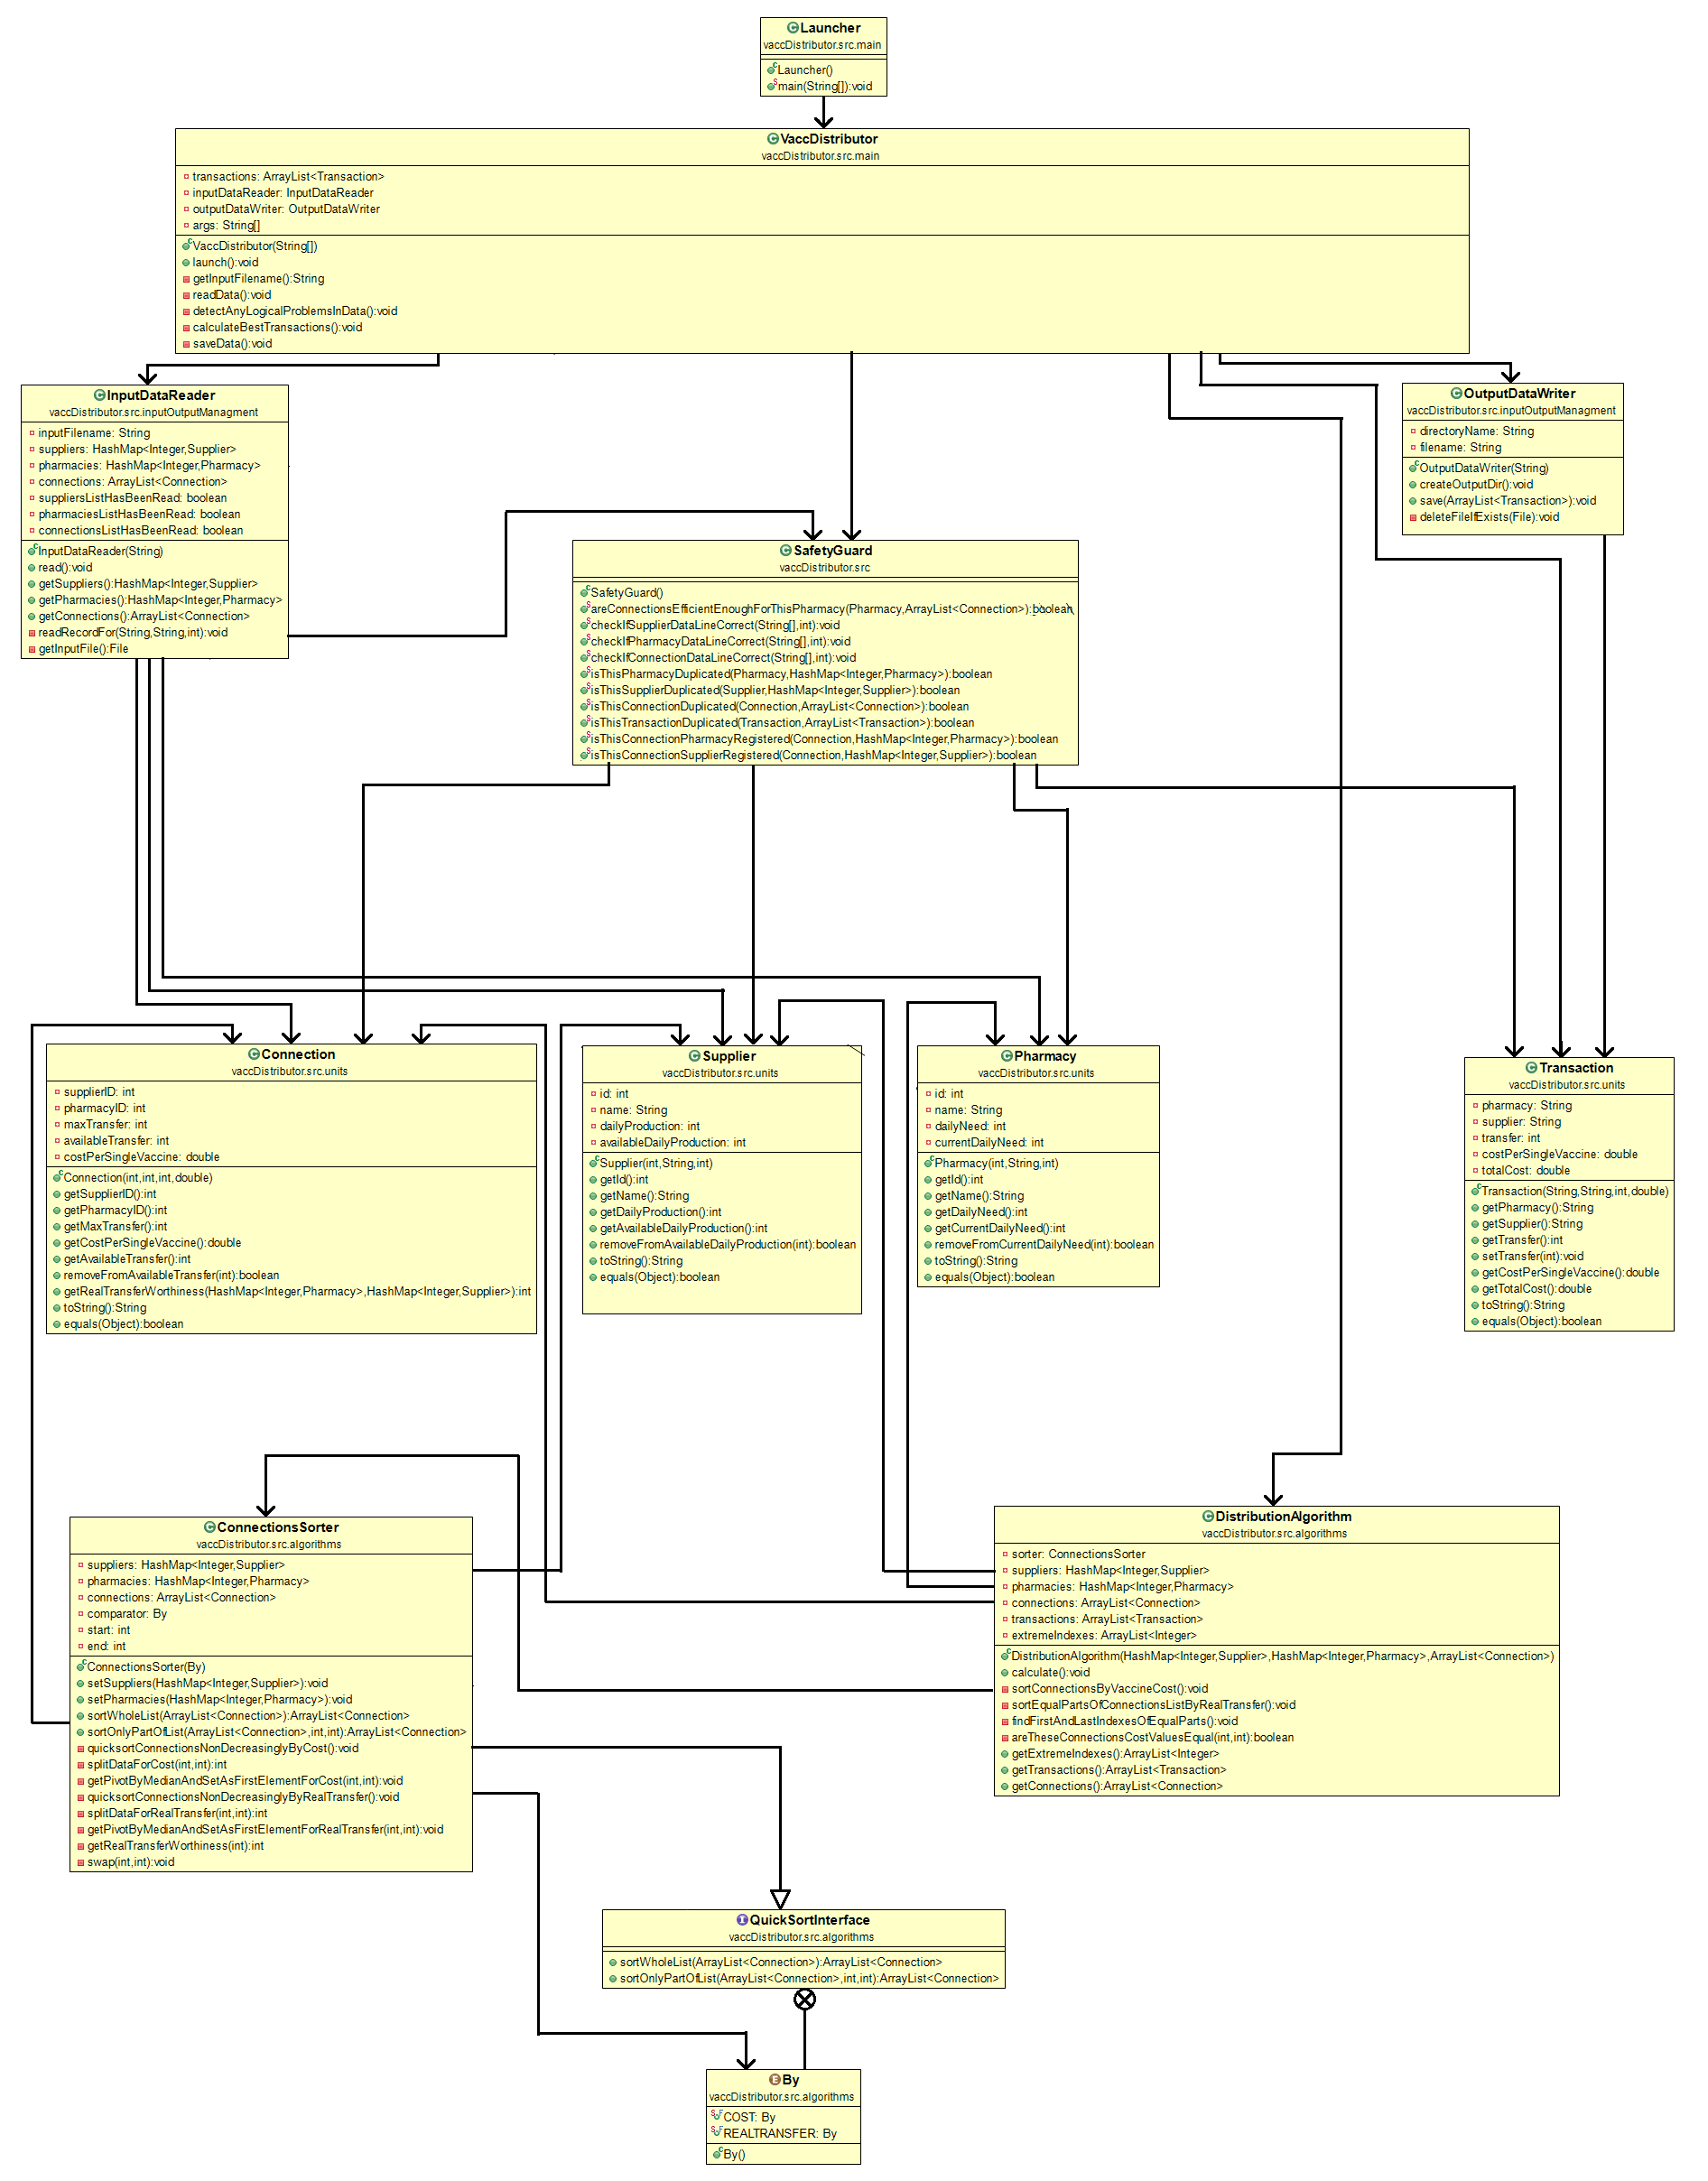
\includegraphics[width=15cm]{Diagram.png}
    \centering
\end{figure}
\end{document}